% Provenance (never printed): see sources/outline_sources.md (Year 3:
% planetary atmospheres, escape, the runaway greenhouse, Mars, Titan,
% habitability).
% Brief: sources/book5/BRIEFS.md, ch. 27. Curves from figdata/bachelor-3/
% jeans_escape.py (escape parameter and escaping fraction at the exobases
% of Venus, the Earth, Mars and Titan), runaway_greenhouse.py (an
% illustrative grey model of a moist atmosphere: OLR against surface
% temperature) and habitability.py (the habitable-zone fits of Kopparapu et
% al. 2013; the phase boundaries of water and methane with the surface
% states of four bodies). Exercise and problem values in the Book 5 scratch
% calculator calc/ch27.py. Kepos and its star are invented.
\chapter{Atmósferas planetarias y habitabilidad}\label{ch:b3:planetary-atmospheres}

Venus y la Tierra son casi gemelas: de tamaño casi igual, densidades medias
similares y órbitas vecinas. Sin embargo, Venus conserva \qty{92}{bar} de dióxido de carbono
sobre una superficie a \qty{737}{K}, y tan poca agua que, extendida
sobre su superficie, formaría una capa de apenas un centímetro de espesor. El
espectrómetro de masas de la sonda Pioneer Venus, al descender a través de sus nubes,
midió la razón entre deuterio e hidrógeno en esa agua: \num{0.016},
cien veces la razón de los océanos terrestres. El hidrógeno ligero escapa al
espacio con más facilidad que el deuterio pesado; lo que queda de un gran reservorio
que ha perdido la mayor parte de su hidrógeno está enriquecido en deuterio. La razón es la
huella del agua que Venus tuvo alguna vez y perdió. Este capítulo se pregunta cómo
retiene un planeta su aire y su agua, y cómo los pierde.
% ledger: planet:Venus.diameter, planet:Earth.diameter, planet:Venus.density, planet:Earth.density, nasa:venus-atm, arney18:venus-water, donahue82:dh, kc98:standards

\begin{recall}
La altura de escala, la fórmula barométrica, la distribución de Maxwell--Boltzmann,
la velocidad de escape, el recorrido libre medio y el efecto invernadero
se estudian en los libros de física. La zona habitable de una estrella
aparece en los libros de la escuela. La temperatura de equilibrio y el albedo de Bond
se encuentran en el volumen de primer año, en su capítulo de planetología comparada;
la profundidad óptica, en su capítulo de telescopios y fotometría;
los gradientes térmicos, en su capítulo sobre la estructura de la atmósfera y del océano;
la radiación de onda larga saliente (OLR) y la temperatura de emisión, en su
capítulo sobre radiación y transporte de calor. El adiabato húmedo se encuentra en el volumen de segundo año,
en su capítulo sobre termodinámica atmosférica; la línea de nieve, en su
capítulo sobre formación planetaria; el ciclo largo del carbono y el
termostato de meteorización de silicatos, en su capítulo sobre el clima a lo largo del
tiempo geológico. La \omterm{prop:b3:stable-isotopes:rayleigh-distillation}{destilación de Rayleigh} se estudia en este volumen, en su capítulo sobre
isótopos estables.
\end{recall}

\section{La estructura de una atmósfera}\label{sec:b3:planetary-atmospheres:structure}

Una atmósfera isoterma de masa molecular $m$ a temperatura $T$ se adelgaza
con la altura según $p = p_0\,e^{-z/H}$, con la altura de escala $H = kT/mg$. En
la superficie de la Tierra $H$ es de unos \qty{8}{km}; en la superficie de
Titán, donde la gravedad es débil y el aire frío, de unos \qty{20}{km}.

La temperatura, sin embargo, no es uniforme. La luz solar que llega al suelo
lo calienta; el aire situado encima, que absorbe y emite en el infrarrojo, se
calienta desde abajo. La radiación por sí sola haría que la atmósfera inferior
tuviera un gradiente térmico tan pronunciado que se volcaría.

\begin{definition}[Equilibrio radiativo--convectivo]\label{def:b3:planetary-atmospheres:rce}
Una columna de atmósfera está en \emph{equilibrio radiativo--convectivo
}\index{equilibrio radiativo--convectivo} cuando, en cada nivel,
el flujo neto de radiación está equilibrado, salvo en una capa inferior donde la convección transporta calor hacia arriba
y mantiene el gradiente térmico en el valor adiabático. La capa inferior,
convectiva, es la troposfera; la capa superior, en equilibrio radiativo,
es la estratosfera; la tropopausa
es el nivel donde ambas se encuentran.
\end{definition}

El modelo atmosférico más sencillo en el que puede seguirse este proceso es el \emph{gris}: es
transparente a la luz solar y absorbe por igual todas las longitudes de onda infrarrojas,
con una profundidad óptica $\tau$ contada hacia abajo desde la cima.

\begin{proposition}[Equilibrio radiativo gris]\label{prop:b3:planetary-atmospheres:grey}
En una atmósfera gris en equilibrio radiativo que emite el flujo $F$ hacia el
espacio, la temperatura a la profundidad óptica $\tau$ obedece
\[
\sigma T^4(\tau) = \frac F2\,(1 + D\tau),
\]
donde $D \approx 1.66$ tiene en cuenta las trayectorias oblicuas de la radiación.
La cima de la atmósfera se encuentra a la \emph{temperatura de piel}
$T_\mathrm{skin} = 2^{-1/4}\,T_e$, donde $T_e = (F/\sigma)^{1/4}$ es la
temperatura de emisión.
\end{proposition}

La proposición se admite; se deduce de las ecuaciones de dos corrientes para
los flujos ascendente y descendente. Donde $\tau$ es grande, cerca del suelo,
la temperatura radiativa cambia rápidamente con $\tau$, y el propio $\tau$
crece deprisa con la profundidad porque el gas absorbente es allí más denso: el
perfil radiativo es más empinado que el adiabato, y entra en juego la convección.
En las capas altas, $\tau$ es pequeño y la temperatura tiende a la
temperatura de piel. La Tierra emite hacia el espacio unos \qty{239}{W.m^{-2}}, con
una temperatura de emisión de \qty{255}{K} y una temperatura de piel de
\qty{214}{K}; la atmósfera estándar sitúa su tropopausa a \qty{11}{km}
y \qty{216.65}{K}. El modelo gris, por sencillo que sea, sitúa bastante bien la cima fría de
la troposfera.
% ledger: ipcc:budget-toa, ussa76:sea-level, ussa76:layers, const:sigma

\begin{omfigure}
\centering
\begin{tikzpicture}[x=1cm, y=0.8cm, font=\small]
% temperature profile (schematic)
\draw[->] (0,0) -- (6.8,0) node[below left, font=\scriptsize] {temperatura};
\draw[->] (0,0) -- (0,8.4) node[above, font=\scriptsize] {altura};
\draw[thick, omDef] (5.6,0) -- (4.2,2.0) -- (4.2,2.6) -- (4.7,3.6)
  -- (3.8,4.6) .. controls (4.3,5.6) and (5.9,6.0) .. (6.2,6.6) -- (6.25,8.2);
\draw[dashed, black!50] (0,2.0) -- (6.8,2.0) node[right, font=\scriptsize, black] {tropopausa};
\draw[dashed, black!50] (0,4.6) -- (6.8,4.6) node[right, font=\scriptsize, black] {homopausa};
\draw[thick, red!70!black] (0,6.6) -- (6.8,6.6) node[right, font=\scriptsize] {exobase};
\node[anchor=west, font=\scriptsize] at (0.15,0.9) {troposfera: convección};
\node[anchor=west, font=\scriptsize] at (0.15,0.5) {(adiabato)};
\node[anchor=west, font=\scriptsize] at (0.15,3.2) {estratosfera:};
\node[anchor=west, font=\scriptsize] at (0.15,2.8) {equilibrio radiativo};
\node[anchor=west, font=\scriptsize] at (0.15,5.6) {termosfera};
\node[anchor=west, font=\scriptsize] at (0.15,5.2) {(calentada por EUV)};
\node[anchor=west, font=\scriptsize] at (0.15,7.6) {exosfera:};
\node[anchor=west, font=\scriptsize] at (0.15,7.2) {sin colisiones};
% exosphere trajectories
\begin{scope}[shift={(11.0,0)}]
\fill[black!8] (-2.3,0) rectangle (2.3,6.6);
\draw[red!70!black, thick] (-2.3,6.6) -- (2.3,6.6);
\node[font=\scriptsize] at (0,0.5) {colisiones por todas partes};
\node[font=\scriptsize, align=center] at (0,3.3) {gas mezclado por\\turbulencia por debajo de la\\homopausa, separado\\por difusión molecular por encima de ella};
\draw[->, thick, omDef] (-1.6,6.6) .. controls (-1.4,8.0) and (-0.9,8.0) .. (-0.7,6.6);
\node[font=\scriptsize, omDef] at (-1.15,8.3) {balística};
\draw[->, thick, red!70!black] (0.4,6.6) -- (1.2,8.5);
\node[font=\scriptsize, red!70!black, anchor=west] at (1.25,8.3) {escapando};
\node[font=\scriptsize, align=center, anchor=north] at (0,6.45) {$v > v_\mathrm{esc}$ hacia arriba:\\ perdida al espacio};
\end{scope}
\end{tikzpicture}
\par\smallskip{\small Las capas de una atmósfera planetaria (esquema, no
a escala). A la izquierda: un perfil de temperatura semejante al terrestre, con la
troposfera fijada al adiabato por la convección, una estratosfera en
equilibrio radiativo y una termosfera calentada desde arriba por la luz solar
ultravioleta extrema. A la derecha: por encima de la \omterm{def:b3:planetary-atmospheres:exobase}{exobase} una partícula no
encuentra nada; una que se mueve hacia arriba más deprisa que la velocidad de
escape abandona el planeta, y una más lenta cae de nuevo siguiendo un arco balístico.}\label{fig:b3:planetary-atmospheres:structure}
\end{omfigure}
% ledger: gronoff:exobase, gronoff:diffusion

En lo alto de la atmósfera el aire es tan tenue que una molécula puede recorrer
una gran distancia entre colisiones. Donde puede recorrer más que una altura de escala, deja de
pertenecer a un fluido.

\begin{definition}[Exobase; exosfera]\label{def:b3:planetary-atmospheres:exobase}
La \emph{exobase}\index{exobase} de una atmósfera es el nivel en el que
el recorrido libre medio de sus partículas iguala a la altura de escala. Por encima de ella,
la \emph{exosfera}\index{exosfera}, una partícula que se mueve hacia arriba es
poco probable que encuentre otra, y una más rápida que la velocidad de escape local
abandona el planeta.
\end{definition}

\begin{proposition}[Condición de la exobase]\label{prop:b3:planetary-atmospheres:exobase}
En una atmósfera isoterma de partículas de sección eficaz de colisión
$\sigma_c$, una partícula que se mueve verticalmente hacia arriba desde el nivel de densidad
$n$ evita toda colisión con probabilidad $e^{-n\sigma_c H}$. En la
\omterm{def:b3:planetary-atmospheres:exobase}{exobase} $n\sigma_c H = 1$: la probabilidad es $1/e$.
\end{proposition}

\begin{proof}
A lo largo de un tramo $\mathrm dz$ la partícula encuentra de media $n(z)\sigma_c\,
\mathrm dz$ otras. La probabilidad de no encontrar ninguna en el ascenso desde
$z_0$ es $\exp(-\sigma_c\int_{z_0}^\infty n\,\mathrm dz)$, y en una
atmósfera isoterma $\int_{z_0}^\infty n_0\,e^{-(z-z_0)/H}\,\mathrm dz
= n_0 H$. El recorrido libre medio es $\ell = 1/n\sigma_c$; la condición $\ell
= H$ es $n\sigma_c H = 1$.
\end{proof}

La \omterm{def:b3:planetary-atmospheres:exobase}{exobase} se encuentra a unos \qty{500}{km} en la Tierra, \qty{200}{km} en
Venus y en Marte, y cerca de \qty{1500}{km} en Titán, más de la mitad del
radio de la luna.
% ledger: gronoff:exobases

\section{Escape atmosférico}\label{sec:b3:planetary-atmospheres:escape}

En la \omterm{def:b3:planetary-atmospheres:exobase}{exobase} las partículas conservan la distribución de Maxwell--Boltzmann de
velocidades del gas inferior. Su cola contiene siempre algunas partículas más rápidas que
la velocidad de escape.

\begin{definition}[Escape de Jeans; parámetro de escape]\label{def:b3:planetary-atmospheres:jeans-escape}
El \emph{escape de Jeans}\index{escape de Jeans} es la pérdida hacia el espacio de las
partículas de la cola de Maxwell--Boltzmann que se mueven hacia arriba en la \omterm{def:b3:planetary-atmospheres:exobase}{exobase}
más deprisa que la velocidad de escape. El \emph{parámetro de
escape}\index{parámetro de escape} de partículas de masa $m$ en la \omterm{def:b3:planetary-atmospheres:exobase}{exobase},
de radio $r$ y temperatura $T$, en un planeta de masa $M$, es
\[
\lambda = \frac{GMm}{kTr} = \frac{v_\mathrm{esc}^2}{u^2},
\qquad u = \sqrt{\frac{2kT}m},
\]
la razón entre su energía de ligadura gravitatoria y $kT$, y también el
cuadrado de la velocidad de escape dividido por la velocidad térmica más probable $u$.
\end{definition}

\begin{theorem}[Flujo de Jeans]\label{thm:b3:planetary-atmospheres:jeans}
En una \omterm{def:b3:planetary-atmospheres:exobase}{exobase} de densidad $n$, el número de partículas que escapan por unidad
de área y por unidad de tiempo es
\[
\Phi_\mathrm J = \frac{n\,u}{2\sqrt\pi}\,(1 + \lambda)\,e^{-\lambda}.
\]
\end{theorem}

\begin{proof}
La distribución de velocidades de Maxwell--Boltzmann es $f(\vec v) =
n\,(\pi u^2)^{-3/2}\,e^{-v^2/u^2}$. Una partícula de velocidad $v$ que se mueve formando el
ángulo $\theta$ con la vertical atraviesa una unidad de área horizontal a
un ritmo $v\cos\theta$. Contando solo las velocidades hacia arriba ($0 \le \theta \le
\pi/2$) superiores a $v_\mathrm{esc}$,
\[
\Phi_\mathrm J = \frac{n}{\pi^{3/2}u^3}\int_0^{2\pi}\!\!\mathrm d\varphi
\int_0^{\pi/2}\!\!\cos\theta\sin\theta\,\mathrm d\theta
\int_{v_\mathrm{esc}}^\infty v^3e^{-v^2/u^2}\,\mathrm dv
= \frac{n}{\pi^{3/2}u^3}\cdot2\pi\cdot\frac12\cdot
\frac{u^4}2\,(1 + \lambda)\,e^{-\lambda},
\]
donde la última integral se obtiene mediante el cambio $s = v^2/u^2$ y
una integración por partes: $\int_\lambda^\infty s\,e^{-s}\,\mathrm ds =
(1 + \lambda)e^{-\lambda}$. Agrupando, $\Phi_\mathrm J = n u (1 +
\lambda) e^{-\lambda}/(2\sqrt\pi)$.
\end{proof}

El factor $n u/2\sqrt\pi$ es el flujo de todas las partículas que cruzan
la \omterm{def:b3:planetary-atmospheres:exobase}{exobase} hacia arriba; $(1 + \lambda)e^{-\lambda}$ es la fracción de ellas
que escapan. Decae exponencialmente con la masa de la partícula, ya que
$\lambda \propto m$. En la \omterm{def:b3:planetary-atmospheres:exobase}{exobase} de la Tierra, a \qty{1000}{K}, el hidrógeno
tiene $\lambda = 7.0$ y escapa a un ritmo del 0.7\,\% de su flujo
ascendente; el deuterio, $\lambda = 14$, a \num{1.2e-5}; el helio, $\lambda = 28$,
a \num{2e-11}; el oxígeno, $\lambda = 111$, no escapa en absoluto. En la \omterm{def:b3:planetary-atmospheres:exobase}{exobase} de
Venus, más fría y igual de profunda en el pozo gravitatorio, $\lambda = 22$ incluso para
el hidrógeno; en Marte $\lambda = 5.4$; en Titán $\lambda = 1.5$ para el hidrógeno
y 3.0 para el hidrógeno molecular.
% ledger: gronoff:jeans, gronoff:jeans-table, gronoff:exobases

\begin{omfigure}
\centering
\begin{tikzpicture}
\begin{axis}[name=lam, width=0.47\linewidth, height=0.46\linewidth,
  xmin=0.5, xmax=50, ymin=0.5, ymax=2000, xmode=log, ymode=log,
  xlabel={masa de la partícula (u)}, ylabel={parámetro de escape $\lambda$},
  tick label style={font=\scriptsize}, label style={font=\small},
  xtick={1,2,4,16,28,44}, xticklabels={1,2,4,16,28,44},
  title={(a)}, title style={font=\small},
  legend style={font=\scriptsize, at={(0.5,-0.24)}, anchor=north, legend columns=2, draw=none}]
\fill[black!10] (axis cs:0.5,0.5) rectangle (axis cs:50,2.5);
\node[font=\scriptsize, anchor=east] at (axis cs:40,1.0) {hidrodinámico};
\addplot[thick, orange!80!black] table[x=A, y=Venus] {figdata/out/bachelor-3-jeans_escape-lambda.dat};
\addlegendentry{Venus}
\addplot[thick, omDef] table[x=A, y=Earth] {figdata/out/bachelor-3-jeans_escape-lambda.dat};
\addlegendentry{Tierra}
\addplot[thin, omDef, dashed, forget plot] table[x=A, y=EarthLo] {figdata/out/bachelor-3-jeans_escape-lambda.dat};
\addplot[thin, omDef, dashed, forget plot] table[x=A, y=EarthHi] {figdata/out/bachelor-3-jeans_escape-lambda.dat};
\addplot[thick, red!70!black] table[x=A, y=Mars] {figdata/out/bachelor-3-jeans_escape-lambda.dat};
\addlegendentry{Marte}
\addplot[thick, black!60] table[x=A, y=Titan] {figdata/out/bachelor-3-jeans_escape-lambda.dat};
\addlegendentry{Titán}
\end{axis}
\begin{axis}[at={(lam.east)}, anchor=west, xshift=0.1\linewidth,
  width=0.47\linewidth, height=0.46\linewidth,
  xmin=0, xmax=40, ymin=1e-16, ymax=1, ymode=log,
  xlabel={parámetro de escape $\lambda$}, ylabel={fracción que escapa},
  ytick={1e-16,1e-12,1e-8,1e-4,1},
  tick label style={font=\scriptsize}, label style={font=\small},
  title={(b)}, title style={font=\small}]
\addplot[thick, black] table[x=lam, y=f] {figdata/out/bachelor-3-jeans_escape-factor.dat};
\addplot[only marks, mark=*, mark size=1.8pt, omDef] table[x=lambdaEarth, y=fEarth] {figdata/out/bachelor-3-jeans_escape-species.dat};
\node[font=\scriptsize, omDef, anchor=south west] at (axis cs:7.0,7.1e-3) {H};
\node[font=\scriptsize, omDef, anchor=south west] at (axis cs:14.0,1.2e-5) {D};
\node[font=\scriptsize, omDef, anchor=south west] at (axis cs:27.9,2.2e-11) {He};
\end{axis}
\end{tikzpicture}
\par\smallskip{\small (a)~El \omterm{def:b3:planetary-atmospheres:jeans-escape}{parámetro de escape} en la \omterm{def:b3:planetary-atmospheres:exobase}{exobase} frente a la
masa de la partícula, para Venus (\qty{290}{K}), la Tierra (\qty{1000}{K};
líneas discontinuas: 800 y \qty{1600}{K}, el intervalo del ciclo solar), Marte
(\qty{270}{K}) y Titán (\qty{180}{K}); por debajo de $\lambda \approx 2.5$
(sombreado) el escape pasa a ser hidrodinámico. (b)~La fracción $(1 +
\lambda)e^{-\lambda}$ del flujo ascendente que escapa, con hidrógeno,
deuterio y helio en la \omterm{def:b3:planetary-atmospheres:exobase}{exobase} de la Tierra; oxígeno, con $\lambda = 111$,
queda muy fuera de escala.}\label{fig:b3:planetary-atmospheres:jeans}
\end{omfigure}
% ledger: gronoff:jeans-table, gronoff:exobases, gronoff:jeans, nasa:venus, planet:Earth.mass, nasa:mars, nasa:titan, const:G, const:kB

Cuando $\lambda$ baja a unas pocas unidades, la imagen de partículas que escapan una a una
de una atmósfera estática deja de valer: la atmósfera superior se expande y fluye
alejándose como un viento. Los modelos sitúan la transición en $\lambda$ entre unos 1.5
y 3.

\begin{definition}[Escape hidrodinámico, no térmico y limitado por difusión]\label{def:b3:planetary-atmospheres:hydrodynamic}
El \emph{escape hidrodinámico}\index{escape hidrodinámico} es la pérdida de una
atmósfera superior que escapa en conjunto, calentada desde arriba, cuando su
\omterm{def:b3:planetary-atmospheres:jeans-escape}{parámetro de escape} es pequeño; el flujo puede arrastrar consigo partículas más pesadas.
El \emph{escape no térmico}\index{escape no térmico} es la pérdida de
partículas aceleradas por procesos distintos del calor: reacciones fotoquímicas
que dan a los fragmentos más energía que la de escape, iones captados
por el campo eléctrico del viento solar, pulverización catódica por iones que impactan
sobre la atmósfera superior, y la salida de iones a lo largo de las líneas del campo magnético.
El \emph{escape limitado por difusión}\index{escape limitado por difusión} es el escape
cuyo ritmo lo fija no la \omterm{def:b3:planetary-atmospheres:exobase}{exobase} sino un nivel más bajo, por el ritmo al que
el gas que escapa puede difundirse hacia arriba a través del gas más pesado situado sobre la
\emph{homopausa}\index{homopausa}, el nivel por encima del cual la difusión
molecular, y no la turbulencia, controla la mezcla.
\end{definition}
% ledger: gronoff:jeans, gronoff:nonthermal, gronoff:diffusion

\begin{proposition}[Límite de difusión]\label{prop:b3:planetary-atmospheres:diffusion}
Un gas ligero de razón de mezcla $f$ y masa molecular $m_i$, que se difunde
a través de un gas más pesado de masa molecular $m_a$ y altura de escala $H_a =
kT/m_a g$ con el parámetro de difusión binaria $b$, no puede ascender más deprisa
que
\[
\Phi_\mathrm{DL} = b\,f\left(\frac1{H_a} - \frac1{H_i}\right)
= \frac{b\,f\,(m_a - m_i)\,g}{kT} \approx \frac{b\,f}{H_a}.
\]
\end{proposition}

\begin{proof}
La teoría cinética (admitida) da el flujo ascendente del gas ligero
respecto del pesado, en una columna isoterma, como $\Phi = -b\,f\,
[\,(1/f)\,\mathrm df/\mathrm dz + 1/H_i - 1/H_a\,]$: el gas ligero
se difunde según su propio gradiente, y su altura de escala propia $H_i$ es mayor
que $H_a$. El flujo es máximo cuando la razón de mezcla es uniforme, $\mathrm
df/\mathrm dz = 0$; el gas que escapa no puede extraerse más deprisa sin que su
razón de mezcla disminuya con la altura. Con $1/H = mg/kT$ se obtienen
las dos formas.
\end{proof}

Para el hidrógeno molecular que asciende a través del dióxido de carbono, $b \approx
\qty{1.2e19}{cm^{-1}.s^{-1}}$ a \qty{200}{K}, y con la gravedad
terrestre el límite es $\Phi_\mathrm{DL} \approx
\num{3.0e13}\,f\,(\qty{200}{K}/T)^{1/4}$ moléculas de $\ce{H2}$ por
centímetro cuadrado y por segundo, contando $f$ todo el hidrógeno como $\ce{H2}$. En
la Tierra actual, el escape de hidrógeno está limitado por difusión: en el
mínimo solar, cuando la \omterm{def:b3:planetary-atmospheres:exobase}{exobase} es más fría y el \omterm{def:b3:planetary-atmospheres:jeans-escape}{escape de Jeans} es más lento, el escape por
intercambio de carga con iones ocupa el hueco, y el total se mantiene
aproximadamente igual. El suministro, y no la
\omterm{def:b3:planetary-atmospheres:exobase}{exobase}, es lo que fija el ritmo.
% ledger: zahnle19:diffusion, gronoff:diffusion, gronoff:rates

\section{Venus y el invernadero desbocado}\label{sec:b3:planetary-atmospheres:venus}

Venus recibe \qty{2601}{W.m^{-2}} del Sol, 1.91 veces la
parte de la Tierra. Sus nubes de ácido sulfúrico reflejan el 77\,\% de ella, así que absorbe
menos que la Tierra; sin embargo, su superficie está a \qty{737}{K} bajo
una atmósfera de \qty{92}{bar}, formada en un 96.5\,\% por dióxido de carbono. Contiene \qty{6e15}{kg} de agua,
frente a \qty{1.4e21}{kg} en la Tierra, unas 30 partes por millón en
volumen por debajo de las nubes.
% ledger: nasa:venus, nasa:venus-atm, arney18:venus-water

Un planeta con océano se mantiene en equilibrio gracias a su radiación saliente. Si
se calienta, se evapora más agua; el vapor de agua es un gas de efecto invernadero, así que la
radiación saliente crece menos que $\sigma T^4$, pero crece, y el
calentamiento se detiene. Hay un límite para ese crecimiento.

\begin{proposition}[Límite radiativo de una atmósfera húmeda]\label{prop:b3:planetary-atmospheres:limit}
Cuando la superficie de un planeta con océano está lo bastante caliente para que el vapor de agua
domine su atmósfera superior, la temperatura allí sigue la
curva de saturación del agua, y la radiación infrarroja hacia el espacio procede de
un nivel de presión fija. Su temperatura y la radiación saliente
dejan de crecer con la temperatura de la superficie.
\end{proposition}

\begin{proof}
En una columna saturada dominada por vapor, la presión $p$ en cada
nivel es la presión de saturación a la temperatura local, $p =
p_\mathrm{sat}(T)$. La radiación hacia el espacio sale de alrededor del nivel
donde la profundidad óptica desde arriba es aproximadamente uno. Para un gas gris de coeficiente
de absorción másico $\kappa$, la profundidad óptica por encima de la presión $p$
es $D\kappa p/g$, de modo que ese nivel se sitúa en $p_1 = g/D\kappa$, sea cual sea la
temperatura de la superficie, y su temperatura es la que cumple
$p_\mathrm{sat}(T) = p_1$. Calentar la superficie solo añade vapor por debajo de ese nivel.
\end{proof}

\begin{definition}[Invernadero desbocado; límite del invernadero desbocado; invernadero húmedo]\label{def:b3:planetary-atmospheres:runaway}
El \emph{límite del invernadero desbocado}\index{límite del invernadero desbocado} es el
mayor flujo de radiación infrarroja que un planeta con océano puede enviar al
espacio. Un \emph{invernadero desbocado}\index{invernadero desbocado} es el estado
de un planeta que absorbe más luz solar que ese límite: no puede equilibrar
su balance hasta que todo el océano se haya evaporado y la superficie se haya
calentado muy por encima de ese valor. Un \emph{invernadero húmedo}\index{invernadero húmedo}
es el estado de un planeta, sin llegar al desbocado, cuya superficie es lo bastante cálida
para que su estratosfera contenga una gran razón de mezcla de vapor de agua,
que la luz ultravioleta descompone y cuyo hidrógeno escapa.
\end{definition}

Los modelos simples, como el de la proposición, dan un límite de este tipo; con las
líneas reales del vapor de agua, un cálculo línea a línea sin nubes
lo sitúa en \qty{291}{W.m^{-2}} para un planeta semejante a la Tierra, y las
revisiones citan unos \qty{300}{W.m^{-2}}. Por encima de unos \qty{2000}{K} el
flujo saliente vuelve a crecer, porque la atmósfera baja caliente emite en el
visible y en el infrarrojo cercano, donde el agua absorbe poco: un planeta en un
\omterm{def:b3:planetary-atmospheres:runaway}{invernadero desbocado} se estabiliza a una temperatura muy alta, una vez que su océano
es todo vapor.
% ledger: kopparapu13:runaway, arney18:runaway

\begin{omfigure}
\centering
\begin{tikzpicture}
\begin{axis}[width=0.8\linewidth, height=0.48\linewidth,
  xmin=250, xmax=600, ymin=150, ymax=560,
  xlabel={temperatura superficial (\unit{K})},
  ylabel={flujo (\unit{W.m^{-2}})},
  tick label style={font=\scriptsize}, label style={font=\small}]
\addplot[very thick, omDef] table[x=Ts, y=olr] {figdata/out/bachelor-3-runaway_greenhouse-olr.dat};
\addplot[dashed, black!60, domain=250:600] {291};
\addplot[thick, orange!80!black, domain=250:600] {525};
\addplot[thick, orange!60!black, densely dotted, domain=250:600] {367};
\addplot[thick, black!70, densely dashed, domain=250:600] {238};
\node[font=\scriptsize, black!60, anchor=south east] at (axis cs:595,291) {límite de línea a línea, \qty{291}{W.m^{-2}}};
\node[font=\scriptsize, orange!80!black, anchor=south east] at (axis cs:595,525) {Venus hoy, sin nubes};
\node[font=\scriptsize, orange!60!black, anchor=south east] at (axis cs:595,367) {Venus joven, Sol al 70\,\%};
\node[font=\scriptsize, black!70, anchor=north east] at (axis cs:595,236) {la Tierra hoy};
\node[font=\scriptsize, omDef, anchor=west] at (axis cs:264,212) {radiación saliente (modelo)};
\end{axis}
\end{tikzpicture}
\par\smallskip{\small Radiación infrarroja saliente de un planeta oceánico semejante a la Tierra
planeta frente a su temperatura superficial, en un modelo gris ilustrativo
(una adiabática húmeda saturada sobre 1~bar de nitrógeno, una estratosfera a
\qty{200}{K}, el vapor de agua como único absorbente; su coeficiente de absorción,
ensanchado por la presión, se elige para coincidir con el límite de línea a línea).
Líneas horizontales: la luz solar absorbida por Venus hoy y por un Venus joven
con un albedo de 0.193, el albedo de una atmósfera caliente de vapor sin nubes,
y por la Tierra hoy con su albedo de 0.3. Donde el flujo absorbido
queda por encima de la meseta, ninguna temperatura superficial lo equilibra: el
invernadero se desboca.}\label{fig:b3:planetary-atmospheres:runaway}
\end{omfigure}
% ledger: kopparapu13:runaway, iapws:vapour-pressure, iapws4:sublimation, const:R, const:sigma, nasa:venus, gough81:luminosity, ipcc:budget-toa

Con el albedo de una atmósfera de vapor sin nubes, 0.193, un planeta semejante a la Tierra
alrededor del Sol se desboca cuando recibe 1.06 veces la luz solar terrestre,
a \qty{0.97}{au}. Antes de eso, con 1.015 veces la luz solar terrestre
y una temperatura superficial de \qty{340}{K}, su estratosfera se vuelve húmeda:
en la Tierra actual el agua queda retenida en la tropopausa por el frío, cerca de
\qty{0.1}{bar}, pero en un planeta más cálido la trampa fría asciende y deja pasar el vapor.
Cuando la razón de mezcla del agua en la estratosfera alcanza unas
\num{3e-3}, el \omterm{def:b3:planetary-atmospheres:hydrodynamic}{escape limitado por difusión} elimina un océano de hidrógeno en un tiempo
del orden de la edad de la Tierra.
% ledger: kopparapu13:runaway, kopparapu13:water-loss, arney18:runaway

El deuterio de Venus mide lo que se perdió. Cada átomo que escapa
elimina hidrógeno y un poco de deuterio del reservorio restante, igual que
cada gota que precipita arrastra un poco de los isótopos pesados de una
nube.

\begin{proposition}[Enriquecimiento isotópico por escape]\label{prop:b3:planetary-atmospheres:dh}
Sea un reservorio de agua que pierde hidrógeno hacia el espacio, escapando cada átomo de deuterio
con la eficiencia $\alpha$ respecto de un átomo de hidrógeno
($\alpha < 1$). Cuando el reservorio se ha reducido de $M_0$ a $M$, su razón
$R = \mathrm{D}/\mathrm{H}$ ha crecido de $R_0$ a
\[
\frac R{R_0} = \left(\frac{M_0}M\right)^{1-\alpha}.
\]
\end{proposition}

\begin{proof}
Perder $\mathrm dN_\mathrm H$ átomos de hidrógeno cuesta al reservorio
$\mathrm dN_\mathrm D = \alpha R\,\mathrm dN_\mathrm H$ átomos de deuterio:
$\mathrm dN_\mathrm D/N_\mathrm D = \alpha\,\mathrm dN_\mathrm H/
N_\mathrm H$, así que $N_\mathrm D \propto N_\mathrm H^\alpha$ y $R \propto
N_\mathrm H^{\alpha - 1}$. La masa de agua es proporcional a
$N_\mathrm H$. Esta es la \omterm{prop:b3:stable-isotopes:rayleigh-distillation}{destilación de Rayleigh}, con el escape en lugar de
la lluvia.
\end{proof}

Si no hubiera escapado nada de deuterio ($\alpha = 0$), un enriquecimiento cien veces mayor
significaría que Venus llegó a tener al menos cien veces su agua actual. Un escape que fracciona menos
exige mucho más: en el \omterm{def:b3:planetary-atmospheres:hydrodynamic}{escape limitado por difusión}
$\alpha \approx 0.8$, y un enriquecimiento cien veces mayor requeriría que el reservorio
se redujera en un factor de $100^5$. La razón se lee como una cota inferior:
al menos unas pocas décimas de por ciento de un océano terrestre,
y las estimaciones de un océano primitivo de Venus van de 4 a \qty{525}{m} repartidos
sobre su superficie. Quedan dos advertencias. Gran parte del fraccionamiento pudo producirse
solo en la pérdida de los últimos pocos bares de agua, y un suministro constante
de agua procedente de cometas o volcanes, perdido tan deprisa como llegaba, podría producir
la misma razón. Venus sigue perdiendo agua: sus iones que escapan son hidrógeno y oxígeno
en la proporción de dos a uno, arrastrados por un campo eléctrico
cinco veces más intenso que el de la ionosfera terrestre,
alrededor de un planeta sin campo magnético.
% ledger: donahue82:dh, arney18:venus-water, arney18:runaway, arney18:venus-loss, zahnle19:rayleigh

\section{Marte: una atmósfera delgada y un pasado húmedo}\label{sec:b3:planetary-atmospheres:mars}

Marte conserva una presión superficial media de \qty{6.36}{mbar}, entre 4.0 y
\qty{8.7}{mbar} según las estaciones, un 95\,\% de dióxido de carbono, a unos
\qty{214}{K}. La presión apenas supera la presión del punto triple del
agua, \qty{6.1}{mbar}: el agua líquida no puede mantenerse en su superficie, donde
el hielo sublima. Sin embargo, los terrenos antiguos están surcados por valles ramificados, y
contienen minerales que solo se forman en agua líquida.
% ledger: nasa:mars-atm, iapws:triple-critical, nasa:mars-water, lasp:maven

\begin{omfigure}
\centering
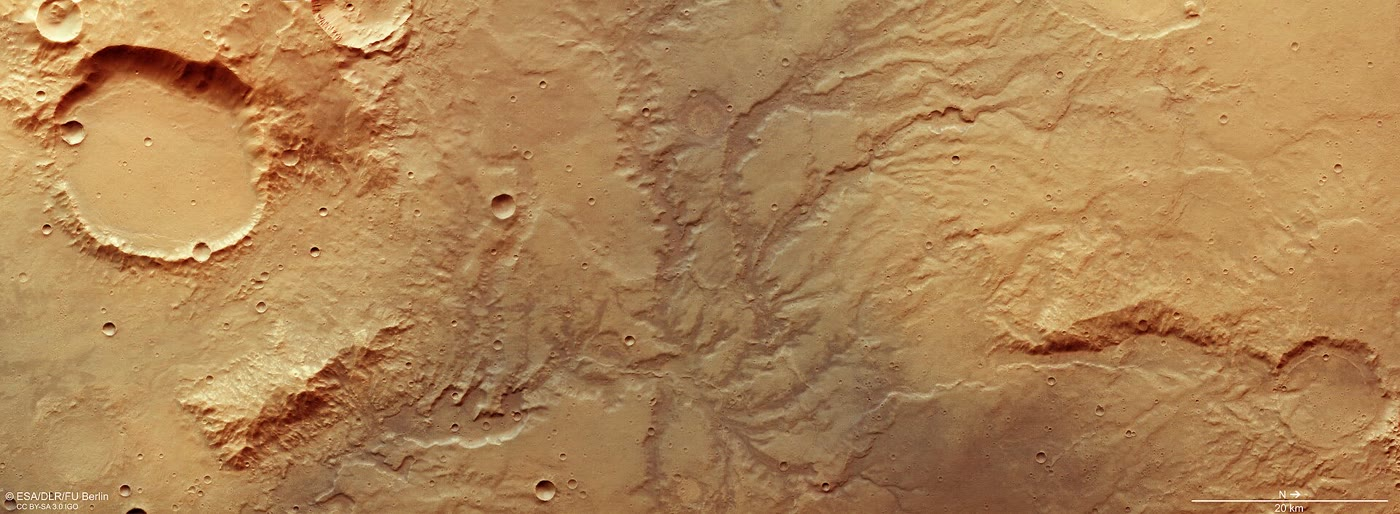
\includegraphics[width=\linewidth]{images/book5/b3-mars-valley-network.jpg}
\par\smallskip{\small Red de valles secos en Marte, vista por la
cámara de Mars Express a unos \qty{14}{m} por píxel, cerca de \ang{17}\,S,
\ang{66}\,E; el norte queda a la derecha, y la barra de escala mide \qty{20}{km}.
Los afluentes se unen aguas abajo en valles mayores, el patrón de una
red de drenaje. Imagen ESA/DLR/FU Berlin, CC BY-SA 3.0 IGO.}\label{fig:b3:planetary-atmospheres:valleys}
\end{omfigure}
% ledger: photo:b3-mars-valley-network

Los valles y los canales de flujo de Marte requieren, según las estimaciones geológicas,
una capa global de agua de entre 100 y \qty{1500}{m} de profundidad, frente a 3 a
\qty{25}{m} que hay hoy en su hielo y en su atmósfera. Gran parte del resto se fue al espacio. La
sonda MAVEN midió cómo el viento solar arranca gas de Marte a unos
\qty{100}{g} por segundo, tres cuartas partes de él por la cola que queda
detrás del planeta, donde fluye el viento solar, y una cuarta parte en una pluma
sobre los polos; durante las
tormentas solares de marzo de 2015 la pérdida se aceleró, y probablemente fue mucho
más rápida cuando el Sol joven era más activo. Marte también pierde hidrógeno, unos
\num{3e26} átomos por segundo de media hoy: mantenido durante cuatro mil millones de
años, una pérdida equivalente a una capa global de agua de solo unos \qty{4}{m} de profundidad.
% ledger: gilli25:h-loss, lasp:maven

La tasa no ha sido siempre la actual. La oblicuidad de Marte, \ang{25.2} hoy,
ha oscilado entre 0 y \ang{66} durante los últimos 250 millones de años,
en torno a un valor medio cercano a \ang{35}, mientras que la de la Tierra varía
en poco más de un grado. El movimiento es caótico y no puede reconstruirse hacia atrás durante miles de millones
de años; los cráteres elípticos formados por impactos rasantes, cuyas orientaciones
registran la oblicuidad, sugieren un valor medio de entre unos 10 y \ang{30} durante
los últimos 3.5 mil millones de años aproximadamente. Con oblicuidades altas, el polo de verano se calienta,
asciende más vapor de agua y los modelos climáticos hacen que la pérdida de hidrógeno
sea veinte veces más rápida: a lo largo de la historia de Marte, una capa del orden de
\qty{80}{m}.
% ledger: planet:Mars.obliq, gilli25:obliquity, holo18:obliquity, gilli25:h-loss

\section{Titán: un ciclo de metano}\label{sec:b3:planetary-atmospheres:titan}

Titán, una luna más pequeña que Marte, tiene una atmósfera más densa que la de la Tierra:
una presión superficial alrededor de un 60\,\% mayor, a \qty{-179}{\degreeCelsius}.
La atmósfera está formada por cerca de un 95\,\% de nitrógeno y un 5\,\% de metano, y como la
gravedad de la luna es débil, se extiende a una altura diez veces mayor que la de la Tierra,
hasta casi \qty{600}{km}. La luz ultravioleta descompone el metano y el nitrógeno
en las capas altas; los fragmentos se recombinan en una neblina anaranjada de hidrocarburos más pesados
que oculta la superficie a la luz visible. Por debajo de la neblina,
el metano desempeña el papel del agua: se condensa en nubes, llueve, excava cauces fluviales
y llena lagos y mares de metano y etano.
% ledger: nasa:titan-surface, nasa:titan-facts

\begin{omfigure}
\centering
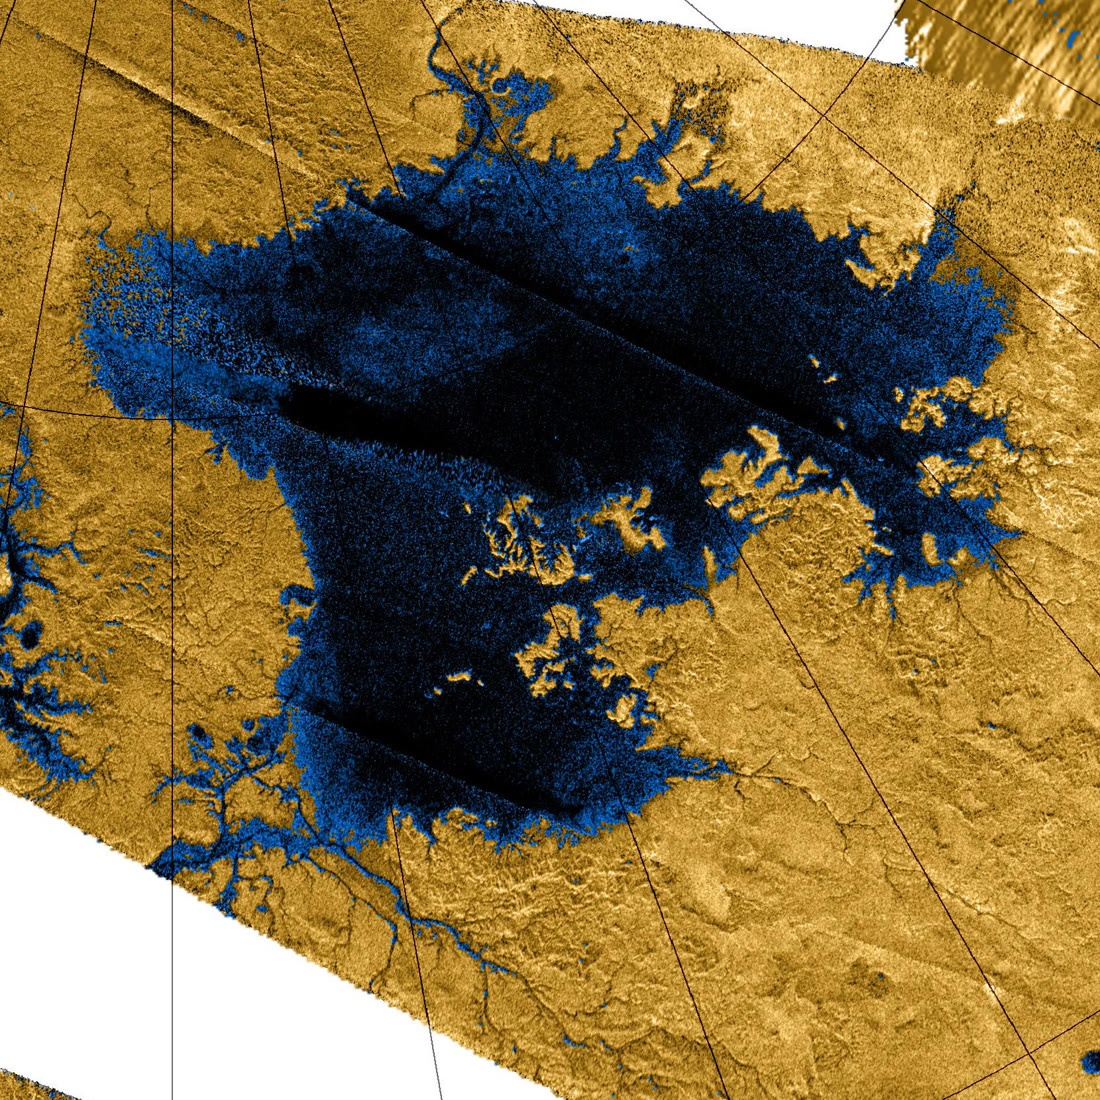
\includegraphics[width=0.5\linewidth]{images/book5/b3-ligeia-mare.jpg}
\par\smallskip{\small Ligeia Mare, un mar próximo al polo norte de Titán, en un
mosaico en falso color de imágenes de radar de Cassini: los rasgos que se cree que son
líquidos aparecen en azul y negro, y el terreno sólido, teñido de marrón, con bahías, islas
y presuntas redes de afluentes. De unos 400 lagos y mares del
norte cartografiado, los de más de \qty{26000}{km^2} concentran el 70\,\% de la superficie.
NASA/JPL/USGS, dominio público.}\label{fig:b3:planetary-atmospheres:ligeia}
\end{omfigure}
% ledger: photo:b3-ligeia-mare

Que un líquido pueda yacer sobre una superficie depende de su diagrama de fases y de la
presión y la temperatura reinantes allí. La superficie de Titán queda justo por encima del
punto triple del metano, \qty{90.67}{K} y \qty{0.117}{bar}, y por debajo de
su punto crítico: es posible el metano líquido, y el metano al 5\,\% de
\qty{1.6}{bar} no está lejos de la saturación. La superficie de Marte se sitúa cerca del
punto triple del agua, la de la Tierra bien dentro de su campo líquido, y
la de Venus, por encima de la temperatura crítica del agua, \qty{647}{K}, donde
no puede existir líquido alguno.
% ledger: nist:methane-phase, iapws:triple-critical, nasa:titan-surface

\begin{omfigure}
\centering
\begin{tikzpicture}
\begin{axis}[width=0.8\linewidth, height=0.52\linewidth,
  xmin=60, xmax=800, ymin=1e-4, ymax=1000, ymode=log,
  xlabel={temperatura (\unit{K})}, ylabel={presión (\unit{bar})},
  tick label style={font=\scriptsize}, label style={font=\small}]
\addplot[thick, omDef] table[x=T, y=p_bar] {figdata/out/bachelor-3-habitability-water.dat};
\addplot[thick, omDef, dashed] table[x=T, y=p_bar] {figdata/out/bachelor-3-habitability-ice.dat};
\addplot[thick, orange!80!black] table[x=T, y=p_bar] {figdata/out/bachelor-3-habitability-methane.dat};
\addplot[only marks, mark=*, mark size=1.6pt, omDef] coordinates {(273.16,0.00611657) (647.096,220.64)};
\addplot[only marks, mark=*, mark size=1.6pt, orange!80!black] coordinates {(90.67,0.1169) (190.6,46.1)};
\addplot[only marks, mark=square*, mark size=2.2pt, black] table[x=T, y=p_bar] {figdata/out/bachelor-3-habitability-bodies.dat};
\node[font=\scriptsize, anchor=south] at (axis cs:737,110) {Venus};
\node[font=\scriptsize, anchor=west] at (axis cs:300,1.0) {Tierra};
\node[font=\scriptsize, anchor=north] at (axis cs:214,0.0045) {Marte};
\node[font=\scriptsize, anchor=south] at (axis cs:94,2.2) {Titán};
\node[font=\scriptsize, omDef, anchor=west] at (axis cs:420,3) {agua: líquido arriba, vapor abajo};
\node[font=\scriptsize, omDef, anchor=north east] at (axis cs:195,0.0012) {hielo};
\node[font=\scriptsize, orange!80!black, anchor=west] at (axis cs:196,46) {metano};
\node[font=\scriptsize, omDef, anchor=south east] at (axis cs:640,230) {punto crítico};
\end{axis}
\end{tikzpicture}
\par\smallskip{\small Los límites entre el vapor y el agua condensada
(en azul: líquido--vapor, desde el punto triple hasta el punto crítico;
a trazos: hielo--vapor) y entre el metano líquido y su vapor (en naranja),
con los estados medios de la superficie de Venus, la Tierra, Marte y Titán
(cuadrados). Un líquido puede yacer sobre una superficie cuya presión supera la
curva de ese líquido, entre sus temperaturas
triple y crítica.}\label{fig:b3:planetary-atmospheres:phases}
\end{omfigure}
% ledger: iapws:vapour-pressure, iapws4:sublimation, iapws:triple-critical, nist:methane-phase, nasa:venus-atm, planet:Earth.Tmean, planet:Earth.psurf, nasa:mars-atm, nasa:titan-surface

Titán retiene su nitrógeno con facilidad: en su \omterm{def:b3:planetary-atmospheres:exobase}{exobase}, $\lambda = 41$ para
el nitrógeno. Su hidrógeno, con $\lambda$ en torno a 1.5, escapa casi libremente, y
el escape del hidrógeno molecular queda fijado más abajo por el flujo limitante
a través de la \omterm{def:b3:planetary-atmospheres:hydrodynamic}{homopausa}, como en la Tierra. Los compuestos pesados formados a partir del
metano descompuesto se depositan en la superficie, donde forman la arena de vastos
campos de dunas.
% ledger: gronoff:jeans-table, gronoff:diffusion, nasa:titan-surface

\section{Habitabilidad planetaria}\label{sec:b3:planetary-atmospheres:habitability}

La zona habitable de los libros escolares es el intervalo de distancias a una
estrella en el que un planeta como la Tierra puede mantener agua líquida en su
superficie. Sus bordes son los límites vistos en este capítulo.

\begin{definition}[Habitabilidad planetaria]\label{def:b3:planetary-atmospheres:habitability}
La \emph{habitabilidad planetaria}\index{habitabilidad planetaria} de un
planeta es su capacidad para mantener agua líquida en su superficie a lo largo de
tiempos geológicos: recibe un flujo estelar dentro de los límites de la
zona habitable, retiene su atmósfera y su agua frente al escape, y un
ciclo del carbono a largo plazo regula su clima.
\end{definition}

El borde interior de la zona habitable lo marca el \omterm{def:b3:planetary-atmospheres:runaway}{invernadero húmedo} o el
\omterm{def:b3:planetary-atmospheres:runaway}{invernadero desbocado}: un planeta semejante a la Tierra alrededor del Sol se vuelve húmedo a
\qty{0.99}{au} y se desboca a \qty{0.97}{au}. El borde exterior lo marca el
\emph{invernadero máximo}: añadir dióxido de carbono calienta un planeta solo hasta que
el gas añadido dispersa más luz solar de la que su efecto invernadero
logra ganar; alrededor del Sol esto ocurre a
\qty{1.70}{au}, con unos \qty{8}{bar} de dióxido de carbono. Estos son
bordes conservadores, calculados sin nubes. Dos bordes empíricos son más amplios:
Venus parece no haber tenido agua superficial durante al menos mil millones de años,
cuando recibió 1.76 veces la luz solar actual de la Tierra (\qty{0.75}{au});
Marte tuvo agua corriente cuando recibió 0.32 veces esa luz solar, si sus
valles tienen 3.8 mil millones de años (\qty{1.77}{au}). Alrededor de estrellas más frías, los mismos límites se dan
con flujos menores, porque su luz más rojiza se dispersa menos y es absorbida
más por el agua y el dióxido de carbono.
% ledger: kopparapu13:runaway, kopparapu13:outer, kopparapu13:hz-fit

\begin{omfigure}
\centering
\begin{tikzpicture}
\begin{axis}[width=0.8\linewidth, height=0.5\linewidth,
  xmin=0, xmax=2.1, ymin=2600, ymax=7200, x dir=reverse,
  xlabel={flujo estelar recibido / el actual de la Tierra},
  ylabel={temperatura estelar (\unit{K})},
  tick label style={font=\scriptsize}, label style={font=\small},
  legend style={font=\scriptsize, at={(0.5,-0.24)}, anchor=north, legend columns=2, draw=none}]
\addplot[name path=mg, thick, omDef] table[x=mg, y=Teff] {figdata/out/bachelor-3-habitability-hz.dat};
\addlegendentry{invernadero húmedo}
\addplot[name path=maxg, thick, red!70!black] table[x=maxg, y=Teff] {figdata/out/bachelor-3-habitability-hz.dat};
\addlegendentry{invernadero máximo}
\addplot[thin, omDef, dashed] table[x=rg, y=Teff] {figdata/out/bachelor-3-habitability-hz.dat};
\addlegendentry{invernadero desbocado}
\addplot[thin, black!60, densely dotted] table[x=rv, y=Teff] {figdata/out/bachelor-3-habitability-hz.dat};
\addlegendentry{Venus reciente, Marte primitivo}
\addplot[thin, black!60, densely dotted, forget plot] table[x=em, y=Teff] {figdata/out/bachelor-3-habitability-hz.dat};
\addplot[green!30, opacity=0.5, forget plot] fill between[of=mg and maxg];
\addplot[only marks, mark=*, mark size=2pt, black, forget plot] coordinates {(1.911,5780) (1.0,5780) (0.431,5780)};
\node[font=\scriptsize, anchor=south] at (axis cs:1.911,5800) {Venus};
\node[font=\scriptsize, anchor=west, xshift=2pt] at (axis cs:1.0,5780) {Tierra};
\node[font=\scriptsize, anchor=east, xshift=-2pt] at (axis cs:0.431,5780) {Marte};
\end{axis}
\end{tikzpicture}
\par\smallskip{\small La zona habitable de un planeta de tipo terrestre, según el
flujo estelar que recibe frente a la temperatura de su estrella (sombreado:
entre el \omterm{def:b3:planetary-atmospheres:runaway}{invernadero húmedo} y el invernadero máximo). Punteado: los
límites empíricos obtenidos a partir de Venus reciente y Marte primitivo. Los ajustes son
los de un modelo climático sin nubes, válidos de 2600 a
\qty{7200}{K}.}\label{fig:b3:planetary-atmospheres:hz}
\end{omfigure}
% ledger: kopparapu13:hz-fit, nasa:venus, nasa:mars

La distancia no basta. Un planeta debe retener su atmósfera: uno pequeño
o caliente, cuyo \omterm{def:b3:planetary-atmospheres:jeans-escape}{parámetro de escape} es bajo, pierde su hidrógeno y con él
su agua, y un planeta en un \omterm{def:b3:planetary-atmospheres:runaway}{invernadero húmedo} se seca desde arriba. Debe
además mantener estable su clima durante miles de millones de años mientras su estrella
aumenta su brillo: en la Tierra, el termostato de meteorización de silicatos del
ciclo del carbono a largo plazo extrae dióxido de carbono cuando el clima se calienta
y lo deja acumularse cuando se enfría. En Venus, sin tectónica de placas,
el dióxido de carbono desgasificado no ha tenido camino de vuelta a las rocas y se ha
acumulado en el aire; hoy contiene aproximadamente tanto dióxido de carbono como el que
la Tierra tiene fijado en rocas carbonatadas. Si un campo magnético protege una
atmósfera es objeto de debate: apantalla la atmósfera superior frente al
viento solar, pero también abre otras vías de escape, como la salida de iones
cerca de los polos, y la habitabilidad de un planeta no puede leerse a partir de su
posición en la zona habitable por sí sola.
% ledger: arney18:venus-loss, gronoff21:magnetic, gronoff:nonthermal

\section{Ejercicios}

\begin{exercise}[$\star$]\label{exo:b3:planetary-atmospheres:1}
Calcúlese la altura de escala $H = RT/Mg$ cerca de la superficie de Venus
(\qty{737}{K}, dióxido de carbono de masa molar \qty{44.01}{g.mol^{-1}},
$g = \qty{8.87}{m.s^{-2}}$), la Tierra (\qty{288}{K},
\qty{28.97}{g.mol^{-1}}, \qty{9.80}{m.s^{-2}}), Marte (\qty{214}{K},
\qty{43.34}{g.mol^{-1}}, \qty{3.71}{m.s^{-2}}) y Titán (\qty{94}{K},
\qty{28.0}{g.mol^{-1}}, \qty{1.35}{m.s^{-2}}). ¿Qué atmósfera es la
más extensa, y por qué?
\end{exercise}

\begin{exercise}[$\star$]\label{exo:b3:planetary-atmospheres:2}
La \omterm{def:b3:planetary-atmospheres:exobase}{exobase} de la Tierra se encuentra a \qty{500}{km} (radio \qty{6878}{km}); su
temperatura varía entre 800 y \qty{1600}{K} a lo largo del ciclo solar. Tómese
la masa de la Tierra como \qty{5.97e24}{kg}. Calcúlese el \omterm{def:b3:planetary-atmospheres:jeans-escape}{parámetro de escape}
de los átomos de hidrógeno a ambas temperaturas, y la fracción de escape
$(1 + \lambda)e^{-\lambda}$. ¿En qué factor la modifica el ciclo solar?
\end{exercise}

\begin{exercise}[$\star$]\label{exo:b3:planetary-atmospheres:3}
Alrededor del Sol, un planeta de tipo terrestre pasa a \omterm{def:b3:planetary-atmospheres:runaway}{invernadero húmedo} con el flujo $S_\mathrm{eff}
= 1.014$, pasa a \omterm{def:b3:planetary-atmospheres:runaway}{invernadero desbocado} con 1.0512 y alcanza el invernadero máximo con 0.3438
(flujos relativos a los de la Tierra). (a)~Calcúlense las tres distancias, en
unidades astronómicas. (b)~Venus y Marte reciben 1.91 y 0.43 veces la
luz solar de la Tierra. Ubíquense.
\end{exercise}

\begin{exercise}[$\star$]\label{exo:b3:planetary-atmospheres:4}
La presión de vapor del metano líquido es $\log_{10}(p/\unit{bar}) = 3.9895 -
443.028/(T/\unit{K} - 0.49)$. (a)~Calcúlese en la superficie de Titán,
\qty{94.15}{K}. (b)~El metano representa el 5\,\% del aire de Titán a \qty{1.6}{bar}.
Calcúlense su presión parcial y su humedad relativa. (c)~¿Qué sugiere
el resultado sobre la evaporación en los mares de Titán?
\end{exercise}

\begin{exercise}[$\star\star$]\label{exo:b3:planetary-atmospheres:5}
En la \omterm{def:b3:planetary-atmospheres:exobase}{exobase} de la Tierra (\qty{1000}{K}, $\lambda = 7.02$ para el hidrógeno),
calcúlese el \omterm{def:b3:planetary-atmospheres:jeans-escape}{parámetro de escape} del deuterio, su velocidad térmica relativa a la del
hidrógeno y la razón de los flujos de Jeans por átomo, D respecto a H. ¿Es el \omterm{def:b3:planetary-atmospheres:jeans-escape}{escape de Jeans}
un filtro isotópico fuerte?
\end{exercise}

\begin{exercise}[$\star\star$]\label{exo:b3:planetary-atmospheres:6}
La razón D/H del agua de Venus es \num{0.016}; la del agua de los océanos en
la Tierra es \num{1.5575e-4}. (a)~Calcúlese el enriquecimiento. (b)~Sin escape
alguno de deuterio, ¿cuál es el inventario pasado mínimo de agua
de Venus, dado \qty{6e15}{kg} hoy? ¿Qué profundidad alcanzaría repartida sobre
la superficie del planeta, \qty{4.60e14}{m^2}? (c)~¿Qué reducción del reservorio
exigiría el \omterm{def:b3:planetary-atmospheres:hydrodynamic}{escape limitado por difusión}, con $\alpha = 0.8$? Conclúyase.
\end{exercise}

\begin{exercise}[$\star\star$]\label{exo:b3:planetary-atmospheres:7}
Marte, de radio \qty{3389.5}{km}, pierde unos \num{3e26} átomos de hidrógeno
por segundo. (a)~Si cada par de átomos procediera de una molécula de agua, ¿qué
capa global de agua elimina esa pérdida en cuatro mil millones de años?
(b)~La misma pregunta para \num{6e27} átomos por segundo, la tasa de una
oblicuidad alta. (c)~Compárese con los 100 a \qty{1500}{m} que
necesitan los valles y los canales.
\end{exercise}

\begin{exercise}[$\star\star$]\label{exo:b3:planetary-atmospheres:8}
(a)~Calcúlese la masa de la atmósfera de Marte a partir de su presión
superficial media, \qty{636}{Pa}, su gravedad, \qty{3.71}{m.s^{-2}}, y su
radio. (b)~El viento solar despoja unos \qty{100}{g} de gas por segundo.
¿Qué masa elimina en cuatro mil millones de años, y en cuánto tiempo
eliminaría la atmósfera actual? (c)~¿Por qué esto es una subestimación de la
pérdida pasada?
\end{exercise}

\begin{exercise}[$\star\star$]\label{exo:b3:planetary-atmospheres:9}
Un planeta semejante a la Tierra, con una atmósfera de vapor de agua sin nubes, refleja el 19.3\,\%
de la luz solar que recibe; su emisión infrarroja no puede superar
\qty{291}{W.m^{-2}}. (a)~¿Por encima de qué flujo de luz solar, en vatios por metro
cuadrado y relativo al de la Tierra, \qty{1361}{W.m^{-2}}, entra en un \omterm{def:b3:planetary-atmospheres:runaway}{invernadero desbocado}?
(b)~Compárese con Venus actual, \qty{2601}{W.m^{-2}}, y con Venus primitiva,
bajo un Sol con el 70\,\% de su luminosidad actual. (c)~¿Por qué no es definitiva
la conclusión para Venus primitiva?
\end{exercise}

\begin{exercise}[$\star\star\star$]\label{exo:b3:planetary-atmospheres:10}
Una termosfera modelo de oxígeno atómico es isoterma a \qty{1000}{K}, con
$n = \qty{1e16}{m^{-3}}$ a \qty{200}{km}; tómese $g =
\qty{9.21}{m.s^{-2}}$ a esa altura y una sección eficaz de colisión
$\sigma_c = \qty{3e-19}{m^2}$. (a)~Calcúlese la altura de escala del oxígeno.
(b)~Calcúlese la densidad en la \omterm{def:b3:planetary-atmospheres:exobase}{exobase} y la altura de la \omterm{def:b3:planetary-atmospheres:exobase}{exobase}.
(c)~La gravedad disminuye con la altura. ¿Desplaza eso la \omterm{def:b3:planetary-atmospheres:exobase}{exobase} hacia arriba o
hacia abajo?
\end{exercise}

\begin{exercise}[$\star\star\star$]\label{exo:b3:planetary-atmospheres:11}
(a)~Supóngase que la estratosfera terrestre se volviera húmeda, con una razón de
mezcla de vapor de agua de \num{3e-3} (contado como $\ce{H2}$). Con el límite
de difusión de $\num{3.0e13}\,f$ moléculas de $\ce{H2}$ por centímetro cuadrado y
por segundo, a \qty{200}{K}, calcúlese la pérdida de hidrógeno de la
Tierra entera (radio \qty{6371}{km}). (b)~¿Cuánto duraría un océano,
con \qty{1.4e24}{g} de agua? Compárese con la edad de la Tierra.
\end{exercise}

\begin{exercise}[$\star\star\star$]\label{exo:b3:planetary-atmospheres:12}
En una atmósfera superior de vapor puro que absorbe como gas gris, con $\kappa =
\qty{0.005}{m^2.kg^{-1}}$, en un planeta con $g = \qty{9.81}{m.s^{-2}}$
y $D = 1.66$: (a)~calcúlese la presión $p_1$ del nivel radiante;
(b)~Con $p_\mathrm{sat}(T) = \qty{611.657}{Pa}\,\exp[(L/R_v)(1/T_t -
1/T)]$, $L = \qty{2.5e6}{J.kg^{-1}}$, $R_v = \qty{461.5}{J.kg^{-1}.K^{-1}}$,
$T_t = \qty{273.16}{K}$, calcúlense su temperatura y el límite de radiación.
(c)~El límite línea a línea es \qty{291}{W.m^{-2}}. ¿Debe el coeficiente
$\kappa$ efectivo del vapor de agua real ser mayor o menor?
\end{exercise}

\section{Problema: ¿conservará Kepos su agua?}

\begin{problem}[{Problema de fin de semana --- escape y habitabilidad de un
planeta oceánico inventado}]
\label{pb:b3:planetary-atmospheres:1}
Kepos es un planeta inventado de masa \qty{5.2e24}{kg} y radio
\qty{6200}{km}, con océanos y una atmósfera de nitrógeno y dióxido de
carbono. Orbita a \qty{0.60}{au} de una estrella de luminosidad 0.30 veces la
del Sol y temperatura efectiva \qty{4800}{K}. Su \omterm{def:b3:planetary-atmospheres:exobase}{exobase} se sitúa
a \qty{500}{km} sobre la superficie, a \qty{1400}{K}, con
\qty{2e11}{m^{-3}} átomos de hidrógeno; su \omterm{def:b3:planetary-atmospheres:hydrodynamic}{homopausa} está a \qty{200}{K},
donde domina el dióxido de carbono y donde el hidrógeno en todas sus formas
constituye una razón de mezcla $f = \num{1e-3}$, contada como $\ce{H2}$. Un océano terrestre equivale a
\qty{1.4e24}{g} de agua.

\medskip\noindent\textbf{Parte I --- La exobase.}
\begin{enumerate}
\item Calcúlense la gravedad superficial y la densidad media de Kepos.
\item Calcúlese la velocidad de escape en la \omterm{def:b3:planetary-atmospheres:exobase}{exobase}.
\item Calcúlese la velocidad térmica $u = \sqrt{2kT/m}$ de los átomos de hidrógeno, helio y
  oxígeno en la \omterm{def:b3:planetary-atmospheres:exobase}{exobase}.
\item Calcúlense sus \omterm{def:b3:planetary-atmospheres:jeans-escape}{parámetros de escape}.
\item ¿Cuáles de ellos pueden escapar por \omterm{def:b3:planetary-atmospheres:jeans-escape}{escape de Jeans} a un ritmo apreciable?
  ¿Alguno se acerca al régimen hidrodinámico?
\item Durante una juventud activa de su estrella, la \omterm{def:b3:planetary-atmospheres:exobase}{exobase} de Kepos pudo haber
  alcanzado \qty{3000}{K}. ¿Cuál era entonces el \omterm{def:b3:planetary-atmospheres:jeans-escape}{parámetro de escape} del hidrógeno,
  y qué sugiere?
\end{enumerate}

\medskip\noindent\textbf{Parte II --- Escape de Jeans del hidrógeno.}
\begin{enumerate}[resume]
\item Calcúlese la fracción que escapa, $(1 + \lambda)e^{-\lambda}$, para
  el hidrógeno.
\item Calcúlese el flujo de Jeans del hidrógeno, por metro cuadrado y por segundo.
\item Calcúlese el número de átomos de hidrógeno que abandonan toda la \omterm{def:b3:planetary-atmospheres:exobase}{exobase}
  por segundo.
\item ¿Cuántos átomos de hidrógeno contiene un océano terrestre?
\item A este ritmo, ¿cuánto tardaría Kepos en perderlos?
\item Calcúlese el \omterm{def:b3:planetary-atmospheres:jeans-escape}{parámetro de escape} del deuterio y su eficiencia de escape
  relativa al hidrógeno, por átomo.
\end{enumerate}

\medskip\noindent\textbf{Parte III --- El límite de difusión.}
\begin{enumerate}[resume]
\item Calcúlese la altura de escala del dióxido de carbono en la \omterm{def:b3:planetary-atmospheres:hydrodynamic}{homopausa}.
\item El parámetro de difusión binaria del hidrógeno en dióxido de carbono es
  $b = \qty{1.2e19}{cm^{-1}.s^{-1}}$ a \qty{200}{K}. Calcúlese el
  flujo limitado por difusión de $\ce{H2}$, por metro cuadrado y por segundo.
\item Compárese con el límite terrestre, $\num{3.0e13}\,f$ moléculas por
  centímetro cuadrado y por segundo, reescalado por la gravedad.
\item Calcúlese el número de átomos de hidrógeno que el límite de difusión puede
  suministrar a la atmósfera superior de todo el planeta por segundo (tómese el
  área de la superficie).
\item Compárese con la pregunta~9. ¿Qué proceso limita el escape y qué
  le ocurre al hidrógeno de la termosfera?
\item ¿Qué densidad de hidrógeno en la \omterm{def:b3:planetary-atmospheres:exobase}{exobase} permitiría que el \omterm{def:b3:planetary-atmospheres:jeans-escape}{escape de Jeans} transportara
  todo el suministro?
\item ¿Cuánto tardaría Kepos en perder un océano terrestre de hidrógeno en el
  límite de difusión?
\end{enumerate}

\medskip\noindent\textbf{Parte IV --- ¿Está Kepos en la zona habitable?}
\begin{enumerate}[resume]
\item Calcúlese el flujo estelar que recibe Kepos, relativo al de la Tierra.
\item Para una estrella de \qty{4800}{K}, el límite del \omterm{def:b3:planetary-atmospheres:runaway}{invernadero húmedo} está en
  $S_\mathrm{eff} = 0.939$ y el límite del invernadero máximo en 0.290. Calcúlense los
  bordes de la zona habitable, en unidades astronómicas, y sitúese Kepos.
\item ¿En qué factor debe aumentar el brillo de la estrella antes de que Kepos alcance el
  borde interior?
\item Con un albedo de 0.3, calcúlese la luz solar absorbida por Kepos por
  metro cuadrado, y su temperatura de equilibrio. Compárese con el \omterm{def:b3:planetary-atmospheres:runaway}{límite del
  invernadero desbocado}.
\item Si un clima más cálido volviera húmeda la estratosfera de Kepos, con
  $f = \num{3e-3}$, ¿cuánto duraría un océano terrestre?
\item Indíquese el tiempo que tardaría Kepos en perder un océano terrestre de hidrógeno por
  \omterm{def:b3:planetary-atmospheres:hydrodynamic}{escape limitado por difusión}, con $f = \num{1e-3}$, en miles de millones de años,
  con dos cifras significativas.
\end{enumerate}
\end{problem}
% ledger: zahnle19:diffusion, kopparapu13:hz-fit, kopparapu13:runaway, gronoff:jeans, const:G, const:kB, const:NA
